\subsection{Qualificação do processo HVOF}

O método de revestimento HVOF foi descrito na Seção~\ref{sec::desc_hvof}. É um
processo de aplicação de revestimento onde partículas metálicas (com ou sem carbonetos) de
aproximadamente 5 a 60 microns são projetadas através de uma chama supersônica
até a superfície que se deseja metalizar, a fim de aumentar a vida útil dessa
superfície contra os desgastes de corrosão, abrasão, erosão e cavitação.
Utilizando propano como combustível, obtêm-se uma aplicação com as seguintes
características: temperatura de chama 2700° C; velocidade da chama de até 2100
m/s; velocidade de partícula 700 m/s; pressão de combustão 80 PSI.

Com este processo é possível aplicar ligas metálicas com carbonetos produzindo
revestimentos densos, com baixo volume de óxidos, alta adesão ao substrato e
dureza de até 1400 HV(Dureza de Vickers). O processo de HVOF possui os seguintes
elementos:

\begin{itemize}
\item Uma pistola de aplicação, onde é realizada a combustão e projeção do
revestimento contra a superfície das pás. Esta deverá estar montada no robô;
\item \textit{Flowmeter} para controle das pressões e vazões dos gases, onde é
regulada a pressão e vazão do O2, Propano e ar comprimido. Deve ser montado
fora do circuito hidráulico, porém o mais próximo possível da escotilha;
\item Alimentador de pó para a pistola, onde é regulado a vazão de pó que é
alimentado para a pistola de aplicação. Deve ser montado fora do circuito
hidráulico, porém o mais próximo possível da escotilha;
\item Cilindros de proprano (estudar necessidade de vaporizador). Combustível 
do processo;
\item Cilindros de O2: comburente do processo;
\item Cilindros de N2: gás de arraste do pó para a pistola;
\item Compressor e secador de ar para a refrigeração da pistola, próximo ao
\textit{Flowmeter};
\item \textit{Chiller} água gelada para refrigeração da pistola. Deve estar
próxima ao \textit{Flowmeter};
\item Estufa para armazenamento da matéria prima;
\item Transformadores de energia 110V;
\item Bomba para compensar queda de pressão da água;
\item Base com rodízio para movimentação dos equipamentos até a escotilha;
\item Exaustor para controle da umidade, temperatura e concentração de gases;
\end{itemize}
 
O projeto de HVOF \textit{in situ} para UHE Jirau busca solucionar os problemas
descritos na seção~\ref{sec::consideracoes}. Dessa forma, as subseções seguintes
abrangem a acessibilidade e movimentação dos equipamentos ao ambiente da
turbina; os principais tipos de revestimentos que resistam a esses desgastes; e
a forma de preparo da superfície por jateamento.

\subsubsection{Movimentação e acessibilidade}
A Fig.~\ref{fig:proj_hvof_1} detalha o circuito hidráulico da turbina na UHE
Jirau. O caminho às escotilhas são superior e inferior são distintos. A
escotilha superior pode ser alcançada por uma plataforma de acesso às unidades
geradoras (1), e uma descida por meio de ponte rolante (2). O caminho à
escotilha inferior é complexo: há uma escada (3) de
aproximadamente 23 metros até a área de descarga (4); do ponto (4) até o
corredor (5) que leva à escotilha são mais 4.77 metros pelo corredor (6), o qual
possui 2.3 metros de altura; por fim, é preciso subir uma escada (7) com
aproximadamente 6 metros de altura por 1,7 de largura.

\begin{figure}
	\centering
	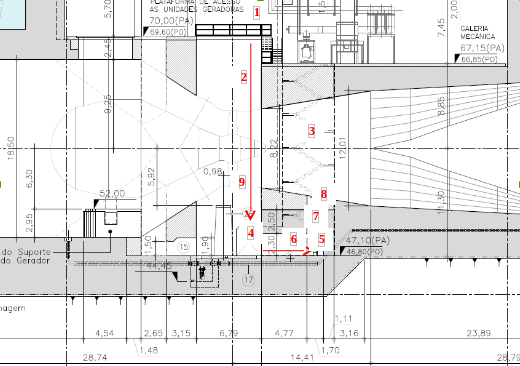
\includegraphics[width=0.7\columnwidth]{sota/figs/projeto/proj_hvof_1.png}
    \caption{Desenho esquema com acesos ao circuito hidráulico.}
    \label{fig:proj_hvof_1}
\end{figure}

A Fig.~\ref{fig:proj_hvof_2} mostra o acesso pela escotilha superior
do aro câmara, e a posição onde os equipamentos podem ficar alocados. A
Fig.~\ref{fig:proj_hvof_3} apresenta o conceito de posicionamento dos
equipamentos levando em consideração o acesso pela escotilha inferior.
Os conceitos de movimentação dos equipamentos são gaiolas para alocação através
de olhais para movimentação vertical e espaço para encaixe de paleteira para
movimentação horizontal dos acesórios para metalização, representados na
Fig.~\ref{fig:proj_hvof_4}.

\begin{figure}
	\centering
	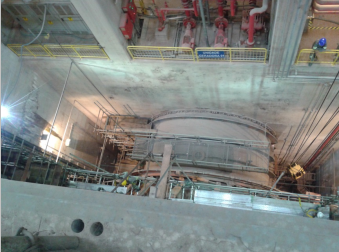
\includegraphics[width=0.7\columnwidth]{sota/figs/projeto/proj_hvof_2.png}
    \caption{Acesso pela escotilha superior do aro câmara.}
    \label{fig:proj_hvof_2}
\end{figure}

\begin{figure}
	\centering
	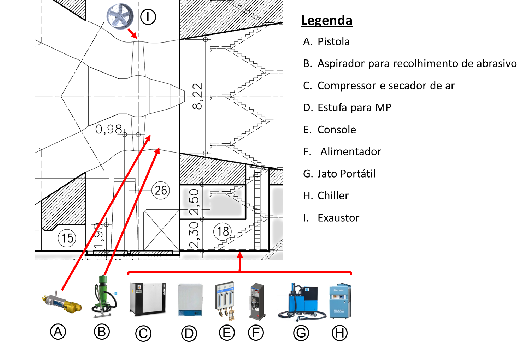
\includegraphics[width=0.9\columnwidth]{sota/figs/projeto/proj_hvof_3.png}
    \caption{Acesso pela escotilha inferior.}
    \label{fig:proj_hvof_3}
\end{figure}

\begin{figure}
	\centering
	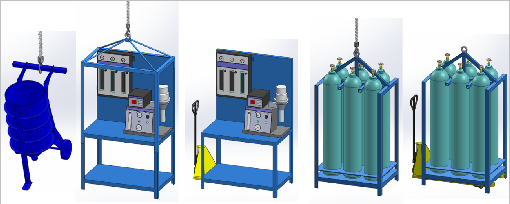
\includegraphics[width=0.7\columnwidth]{sota/figs/projeto/proj_hvof_4.png}
    \caption{Sistemas de movimentação do Jato e eqipamentos acesórios à pistola de Coating.}
    \label{fig:proj_hvof_4}
\end{figure}

\subsubsection{Jateamento abrasivo}

Na Seção~\ref{sec:jat}, o jateamento abrasivo foi introduzido como requisito
para a preparação da superfície a ser revestida. Foram investigados duas
alternativas para posicionamento e a forma de execução do equipamento
para preparação superficial com óxido de alumínio. 

\begin{enumerate}
  \item Máquina de jato com reservatório deverá permanecer fora do circuito
  hidráulico, porém o mais próximo possível da escotilha. A pistola de
  jateamento com recirculação do abrasivo; Compressor de ar com secador:
  secador de ar deve estar próximo a maquina de jato; Sistema de filtragem de
  ar mandado ao operador para abastecer ar filtrado para respiração
  do operador, fora do circuito hidráulico.
  \item Máquina de jato com reservatório do abrasivo deverá permanecer fora do
  circuito hidráulico, porém o mais próximo possível da escotilha. Pistola sem
  sistema de recirculação de abrasivo; Aspirador para recolhimento do abrasivo;
  Compressor de ar com secador ar próximo à maquina de jato; Sistema de
  filtragem de ar mandado ao operador para abastecer ar filtrado
  para respiração, fora do circuito hidráulico.
\end{enumerate}

O jato com sistema recirculante é uma alternativa interessante, porém pode
possuir menor produtividade.

\subsubsection{Tipos de revestimentos}

Para se determinar a solução ideal de revestimento para as pás Kaplan,
primeiramente foram mapeados os principais tipos de desgastes que sofrem os
equipamentos de hidrogeração. Esse mapeamento foi realizado através de estudo
teórico em materiais de fabricantes de equipamentos hidrelétricos, artigos em
revistas científicas e inspeção própria nas unidades geradoras em Jirau. Na
Fig.~\ref{fig:proj_hvof_5}, está apesentada uma das principais regiões
desgastadas pelas pás e os tipos de danos por abrasão, cavitação, erosão e corrosão.

\begin{figure}[h!]
	\centering
	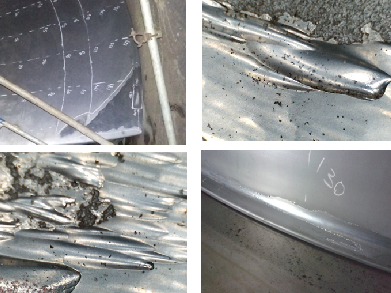
\includegraphics[width=0.9\columnwidth]{sota/figs/projeto/proj_hvof_5.png}
    \caption{Mapeamento do desgaste das pás da UHE Jirau através de inspeção em campo.}
    \label{fig:proj_hvof_5}
\end{figure}

A partir desse mapeamento prévio foram selecionados três tipos de materias para
o revestimento das pás, Tabela~\ref{tab::materiais_HVOF}.

\begin{table}[H]
\centering
\caption{Materiais base para HVOF}
\label{tab::materiais_HVOF}
\begin{tabular}{ccc}
\hline
Sistema                                                                  & Material                                                                                                                                                         & Principal aplicação do revestimento                                                         \\ \hline
\multicolumn{1}{|c|}{WCNiCr}                                             & \multicolumn{1}{c|}{\begin{tabular}[c]{@{}c@{}}Material base em AISI 410 e revestimento de \\ Carboneto de Tungstênio em matriz\\ de Niquel Cromo\end{tabular}}  & \multicolumn{1}{c|}{\begin{tabular}[c]{@{}c@{}}Desgaste\\ Erosivo e Cavitação\end{tabular}} \\ \hline
\multicolumn{1}{|c|}{WCCoCr}                                             & \multicolumn{1}{c|}{\begin{tabular}[c]{@{}c@{}}Material base em AISI 410 e revestimento de \\ Carboneto de Tungstênio em matriz\\ de Cobalto-Cromo\end{tabular}} & \multicolumn{1}{c|}{\begin{tabular}[c]{@{}c@{}}Desgaste\\ Abrasivo e Erosão\end{tabular}}   \\ \hline
\multicolumn{1}{|c|}{\begin{tabular}[c]{@{}c@{}}AISI\\ 410\end{tabular}} & \multicolumn{1}{c|}{\begin{tabular}[c]{@{}c@{}}Material base \\ em aço inoxidável AISI 410\end{tabular}}                                                         & \multicolumn{1}{c|}{---}                                                                    \\ \hline
\end{tabular}
\end{table}

Para qualificar os materiais e as modificações nos equipamentos foram
realizados ensaios baseando-se em procedimentos normatizados. Abaixo é feita a
listagem dos testes realizados bem como a norma a qual aquele teste se
relaciona. Os testes estão classificados em duas categorias: testes para
qualificação do processo, e testes para a seleção do revestimento.

Os testes para qualificação do processo são:

\begin{enumerate}
  \item \textbf{Ensaio de adesão:} Norma Relacionada: ASTM C633; Equipamento
  utilizado: Máquina de ensaios universal; Corpos de prova: 3 corpos de prova
  cilíndricos de 1 polegada de diâmetro para cada conjunto de testes;
  \item \textbf{Microdureza:} Norma Relacionada: ASTM E384; Equipamento
  utilizado: Microdurômetro Vickers com carga de 0.1 à 1 kgf Corpos de prova:
  Retangulares com 25,4 mm x 10 mm x 5 mm. 1 por teste;
  \item \textbf{Medição de Porosidade e Óxidos:} Norma Relacionada: ASTM E2109
  Equipamento utilizado: Microscópio óptico com lentes objetivas de 50 até 1000
 x de aumento. Corpos de prova: Retangulares, os mesmos utilizados para o ensaio
 de microdureza.
  \item \textbf{Rugosidade:} Norma Relacionada: ISO 4287-1997; Equipamento
  utilizado: rugosimetro portátil para medição dos parâmetros Ra, Rz.
  Corpos de prova: serão utilizados os mesmo corpos de prova para o ensaio de
  microdureza.
\end{enumerate}

Os testes para a seleção do revestimento são:
\begin{enumerate}
  \item \textbf{Ensaio de Erosão:} Norma Relacionada: ASTM G76;
  Equipamento utilizado: equipamento de erosão por partículas sólidas;
  Corpos de prova: retangulares com 25,4x15 mm por 5 mm de espessura. Ou 30 mm
   de diâmetro. 3 por teste.
  \item \textbf{Ensaio de Abrasão:} Norma Relacionada: ASTM G65;
  Equipamento utilizado: abrasômetro do tipo roda de borracha;
  Corpos de prova: retangulares de 25,4 x 76 x 5 mm mínimo;
   \item \textbf{Ensaio de Cavitação:} Norma Relacionada: ASTM G32;
    Equipamento utilizado: equipamento de vibração ultrasônico.
   \item \textbf{Ensaio de Imersão – Corrosão:} Norma Relacionada: -//-
   Equipamento utilizado: cuba de imersão e potenciostato;
  Corpos de prova: retangulares com 25,4x20 mm por 5 mm de espessura. 3 por
  teste.
   \item \textbf{Adesão por dobramento:} Norma Relacionada: ASTM B571;
Equipamento utilizado: Dispositiva para dobramento em máquina de ensaio universal
Corpos de prova: 50 x 75 x 3 mm;
\end{enumerate}

\textbf{Demais equipamentos utilizados para controle do processo de
Jateamento e Metalização:}
Termo-higrômetro para medição do ponto de orvalho e controle da umidade relativa do ar;
Pirômetro para controle da temperatura da peça/corpo de prova;
Rugosimetro para medição da rugosidade da superfície jateada e metalizada;
Medidor de camada indutivo para controle da espessura de camada;

\textbf{Accura-Spray para controle da temperatura e velocidade da chama
hipersônica:} Este ensaio é de grande importância para a qualificação dos
procedimentos de HVOF na medida que ele monitora os parâmetros de saída da chama de aspersão
como a temperatura e a velocidade média das partículas. A
Fig.~\ref{fig:proj_hvof_6} mostra o cabeçote do equipamento accura spray
montado próximo à pistola de aspersão para monitoramento de chama.

\begin{figure}
	\centering
	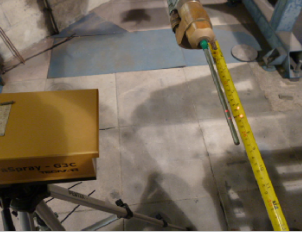
\includegraphics[width=0.7\columnwidth]{sota/figs/projeto/proj_hvof_6.png}
    \caption{Cabeçote do accura spray para monitoramento da chama de aspersão
    témica.}
    \label{fig:proj_hvof_6}
\end{figure}